\chapter{能耗随机混成自动机的验证}
\label{ch4}
\vspace{-0.7cm}
	MARTE/UML采用多视图的方式对系统进行设计、描述,但由于其半形式化的特性,无法实现模型的定性、定量验证。自动机不仅可以刻画系统的行为,且目前已存在很多基于自动机的模型检测方法。本章首先基于随机混成自动机的概念,给出了能耗随机混成自动机的形式化语法和语义,支持显式建模系统中能量的产生与消耗。接着,提出了从MARTE/UML状态图到能耗随机混成自动机的映射规则和转换算法,实现了不可执行模型到到可执行模型的自动转换。最后,基于我们的建模、仿真、验证平台Modana\citep{DBLP:conf/compsac/ChengWLD15,杜德慧2017一种面向}和模型验证工具UPPAAL-SMC\citep{DBLP:journals/spe/BehrmannDLPY11,DBLP:journals/corr/abs-1207-1272},给出了本文所提的智能建筑能耗建模与分析方法的实现框架。
	
\section{能耗随机混成自动机}
\subsection{ESHA的语法}
	随机混成自动机(Stochastic Hybrid Automata,SHA)\citep{Hu2000Towards,David2011Statistical,程贝2016基于抽象和学习的统计模型检测研究}可以被视作添加了随机语义扩展后的混成自动机(Hybrid Automata)\citep{Henzinger1996The}。根据SHA的定义,系统可以由位置(location)和位置间的迁移(transition)描述。在每一个位置上,连续变量随时间的变化速率可能不同,每次迁移可能伴随着系统变量的重新赋值(valuation)。SHA具有混成的语义:在位置上可以利用速率向量(rate vector)来定义连续变量随时钟的变化率;而在位置间的迁移过程中,可以对变量进行重新赋值;同时,SHA也具有随机的语义:位置上可以用时延函数来描述系统在该位置时间延迟的概率;位置之间的迁移可以定义离散的概率值来表示从某个位置发生某个迁移的特定概率。
	
	为了能够显式地描述CPES中的能耗变化,我们在SHA上添加能耗的信息,并且针对能耗产生的不同方式,进行了分类。能耗随机混成自动机的定义如下:
	\begin{myDef}能耗随机混成自动机\end{myDef}	
	一个\textbf{能耗随机混成自动机}(Energy Stochastic Hybrid Automata,ESHA)是一个九元组$ESHA = (L,l_{0},X,\Sigma,T,R,I,F,E)$。
	\begin{itemize}
	\item $L$是位置的有限集合;
	\item $l_{0} \in L$代表初始位置;
	\item $X$是所有变量的集合,包括离散变量、连续变量以及时钟,且时钟的取值范围为 $\mathbb{R^{+}}$;
	\item $\Sigma = \Sigma_{i} \cup \Sigma_{o} $是动作的有限集合,分为输入动作($\Sigma_{i}$)和输出动作($\Sigma_{o}$);
	\item $T \subseteq L \times \Phi(X) \times Prob \times \Sigma \times 2^{X} \times L$是迁移的有限集合,即一个从 $l$ 到 $l^{'}$ 的迁移在输入动作和变量的约束条件下以一定的离散概率发生,并伴随着输出动作和变量的重新赋值;
	\item $R:L\rightarrow \mathbb{N}^X$为每一个位置赋予了一个速率向量来刻画在该位置上连续变量的变化率;
	\item $I : L \rightarrow Inv$ ,其中$Inv$描述了ESHA中位置上的变量约束, $I$定义了这种映射关系;
	\item 对于每一个位置$l \in L$,$f(l)$为该位置上的时延函数。
	\item $E:T \cup L \rightarrow \mathbb{R}$代表ESHA所描述的动态行为过程中的能耗,它将自动机中的每个位置和每条迁移映射到一个实数,来记录相应的能耗,即
	\begin{equation}
	E = E_{t} \cup E_{l}
	\end{equation}
	其中,$E_{t}:T \rightarrow \mathbb{R}$将每个迁移映射到实数上,表示迁移带来的能耗;$E_{l}:L \rightarrow \mathbb{R}$将每个位置映射到实数上,以记录在位置上产生的能耗。迁移和位置上的能耗值均可正可负,能耗值为正代表系统消耗能量,为负代表系统产生能量。
	\end{itemize}
	
\subsection{ESHA的语义}
	SHA的语义可以用一个标签迁移系统描述,在解释ESHA的语义之前,先介绍如下定义。

	\begin{myDef}标签迁移系统\end{myDef}
	一个\textbf{标签迁移系统}(Labeled Transition System,LTS)\citep{DBLP:journals/fm/Trybulec09}是这样一种结构: $\langle S, A, \longrightarrow\rangle$ 
,集合$S$包含系统所有的状态, 集合$A$包含所有标签, 迁移关系 $\longrightarrow\,\subseteq S\times A\times S$。$(s,a,s')\in\longrightarrow$通常表示为$s\stackrel{a}{\longrightarrow}s'$ 。
	
	时钟标签迁移系统是一种标签为时钟集合的标签迁移系统。对于每一个状态,最多有$2^n$条对外的迁移,其中,$n=|C|$表示时钟的数目。每个迁移都可能伴随着时钟的重置。
%A special state, denoted $\bot$, stands for a sink state where the constraint is violated.

	\begin{myDef}时钟标签迁移系统\end{myDef}
	一个\textbf{时钟标签迁移系统}(Clock-labelled Transition System,CLTS)是这样一种结构: $\langle S, C, \longrightarrow\rangle$,其中$\langle S, 2^C, \longrightarrow\rangle$ 是一个标签迁移系统。

	%为了能够建模系统中的能耗,我们通过在每一个位置和迁移上加能耗标注进一步扩展了时钟标签迁移系统,这个扩展后的结构被称作\textbf{能耗时钟标签迁移系统}。
	
	\begin{myDef}能耗随机时钟标签迁移系统\end{myDef}
	基于CLTS,在\citep{DBLP:conf/facs2/DuHJMY16}中我们定义了Probabilistic CLTS的概念,进一步地,可以扩充定义能耗随机时钟标签迁移系统(Energy Stochastic Clock-labelled Transition System,ESCLTS)。ESCLTS是一个特殊的时钟标签迁移系统,其中,$\longrightarrow\ \subseteq (S \cup F \cup E_{l}) \times 2^C \times Prob \times E_t \times (S \cup F \cup E_{l})$。
	
	$F$表示状态$S$处的时延函数,即描述了状态$S$处迁移发生与时间的概率分布关系;$Prob \subseteq \mathbb{R}$是一个[0,1]上的实数,对于一个给定的迁移$t=(s \cup f \cup e_{l},\Gamma,prob,e_{t},s' \cup f' \cup e_{l}^{'})$,$\pi(t)=prob$表示此迁移被触发的概率为$prob$。
	$E_{t(l)}$ 中的元素$e_{t(l)}$代表了某个特定迁移(位置)产生的具体能耗数值。$e_{t(l)}>0$代表系统消耗了能量, $e_{t(l)}<0$代表系统产生了能量。
%type/update

	\begin{myDef}迁移能耗\end{myDef}
\emph{迁移能耗}代表自动机在进行位置迁移时,随之产生的能耗。它由一个三元组来表示:$E_{t} = (Type, Update, \lambda)$,其中,$Type$和$Update$分别表示迁移触发的原因和迁移触发后的后果(包括对系统某些变量的改变)。

	\begin{itemize}
	\item $Type ::= sync | guard$,其中, $sync$ 表示自动机与另一个自动机之间存在消息交互,即由消息触发了迁移;$guard$表示迁移的触发仅仅是由于某个位置上不变式约束条件的违背而造成的。
	\item $Update ::= true | false$ , $true$代表此迁移造成了系统某些变量的重新赋值,而$false$意味着不改变系统的任何变量。
	\end{itemize}

	现在,我们给出$\lambda$的定义,它是系统某次迁移产生的能耗的计算值—— $\lambda:Type \cup Update\rightarrow\mathbb{R}$。在$Type$和$Update$值的不同组合下,$\lambda$的值将有四种计算方式,具体规则如表\ref{energy-transition}所示。

	\begin{table}[!t]
	\renewcommand{\arraystretch}{1.4}
	\caption{迁移能耗的计算}
	\label{迁移能耗的计算}
	\centering
	\begin{tabular}{c c c}
	\hline
	Type & Update & $\lambda$ \\
	\hline
	sync & true & $e_{t}.sync + e_{t}(update)$\\
	sync & false & $e_{t}.sync$\\
	guard & true & $e_{t}(update)$\\
	guard & false & $0$\\
	\hline
	\label{energy-transition}
	\end{tabular}
	\end{table}
 
	根据迁移触发原因的不同,我们来分析ESHA中不同类型迁移所带来的能耗。现实世界中系统不同模块间的信息传递在自动机中被建模为模型间的同步信号。对于特定环境下的系统而言,这种信息传输产生的能耗由线路的物理特性和系统的消息传递机制决定,而与消息的内容无关。因此,可以将每次消息传输的能耗视作一个固定值,记作$e_{t}.sync$。值得注意的是,在ESHA中,一次消息传递被建模为一个模块的信号接收事件和另一个模块的信号发送事件,为了避免能耗的重复计算,可以限定只计算发送事件能耗或只计算接收事件能耗。
	由于不变式条件的违背而产生的迁移,仅仅代表了系统中某些变量值的演化触发了系统的状态迁移,并没有实际动作发生,因此不会带来任何能耗。

	迁移上的$Update$代表对系统中某些变量的赋值,在实际中,这往往意味着系统需要采取一些措施来改变某些变量的值。例如,在一个汽车系统中,``$acceleration =  acceleration +2$''意味着汽车引擎需要加大马力来使得加速度增加两个单位,这一动作会带来额外的能耗。另外,在某些时刻,系统可能需要补充能量,如利用太阳能产生能量,能耗值为负即表示能量的补给。迁移上的赋值操作带来能耗值由具体的动作所决定,故记作$e_{t}(update)$。值得一提的是,在对CPES建模时,由于系统的实时性,常使用时钟来控制某些事件的发生。迁移上可能会伴随着时钟的重置,这实际上是为了建模系统控制而人为设定的,并不耗能。
	
	正如表\ref{迁移能耗的计算}所呈现的,一个离散迁移所产生的能耗为触发事件执行的能耗和动作效应的能耗之和。 对于一个能耗随机时钟标签迁移系统 $\langle S \cup F \cup E_l, 2^{C} \cup E_t, \longrightarrow\rangle$,我们把$e_{t}(t)=e_{t}.\lambda$叫作离散迁移$t \in \longrightarrow$的能耗值。  

\begin{myDef}位置累积能耗\end{myDef}
	位置之间的迁移表示的是系统的离散行为,然而,由于时间的流逝以及系统处于不同位置时能量随时间的变化速率不同,在系统的不同位置,会累积特定的能耗,这种在位置上产生的能耗被称作\textbf{位置累积能耗}。

	位置累积能耗可以通过公式$e_{l}(l) =\int r(t) dt$, s.t. $(l,T)\rightarrow(l,T + \Delta T)$计算而得,其中,$\Delta T$代表了时间流逝的长度,$r(t)$代表在某个位置上能耗随时间的变化率,$(l,T)\rightarrow(l,T + \Delta T)$意味着在某个位置上停留的时间必须使得系统变量满足该位置上的不变式约束。

\begin{myDef}能耗链\end{myDef}
	一条从位置$loc_{1}$到位置$loc_{n}$的能耗链是由位置和迁移的交替排列组成的有向序列,$\gamma = loc_{1,\Delta T_{1}} \xrightarrow{t1} loc_{2,\Delta T_{2}} \xrightarrow{t2} ... \xrightarrow{t(n-1)} loc_{n,\Delta T_{n}}$。尤其需要注意序列的方向,$loc_{1} \xrightarrow{t_{x}} loc_{2}$和$loc_{2} \xrightarrow{t_{y}} loc_{1}$是不同的,因为迁移具有方向性,且不同的迁移带来的能耗不同。一条能耗链的总能耗值是所有迁移能耗和位置累积能耗之和,即
	\begin{equation}
	E(\gamma) = \sum_{i=1}^{n-1}e_{t_{i}}.\lambda + \sum_{i=1}^{n} \int r(t) dt
	\end{equation}
	
	\textbf{最小迁移能耗链}:从位置$loc_{1}$到位置$loc_{n}$通常具有不止一条迁移能耗链,其中,能耗值最小的被称作最小迁移能耗链,即 $\forall \gamma_{l_{1} \rightarrow l_{n}}, E(\gamma_{l_{1} \rightarrow l_{n}}^{min})\leq E(\gamma_{l_{1} \rightarrow l_{n}})$。
		
\section{MARTE模型到ESHA的转换}
	MARTE/UML类图定义了系统的静态元素;顺序图描述了系统为实现某个功能,不同对象之间的交互关系;状态图则更详尽地刻画了对象内部发生的状态变化。状态图与随机混成自动机本质上描述的都是单个对象的动态变化过程,因此,可以基于语义将扩展的MARTE/UML状态图的元素映射为ESHA的元素,实现设计模型到可执行模型的转换,进而对转化得到的模型实现仿真和验证。

\subsection{模型映射规则}
	\textbf{转换的依据}
	
	从建模的基本思想来说,模型是对现实世界的抽象。针对同一个系统,观察的角度和重点不同以及建模的方法不同,都会得到不同的系统模型。但是,当关注的角度相同、针对同样的性质时,不同的建模方法构建出来的系统模型只是表达方式上存在差异,本质上其逻辑语义是一致的\citep{彭大天2013基于}。
	
	\textbf{元素的映射}
	
	根据前述对扩展的MARTE/UML状态图和ESHA的定义,我们给出了如图\ref{SC2ESHA}所示的元素映射规则,其中,ESHA以UPPAAL-SMC工具中的图形化形式表示。UPPAAL-SMC是一个常用的统计模型检测工具,其理论基础是随机混成自动机。本文定义的ESHA可以视作SHA添加了能耗的扩展版本,我们通过自定义特定变量来表示迁移能耗和位置累积能耗。此外,在UPPAAL-SMC中,离散概率选择迁移需要添加Branch节点,且每条迁移的触发概率以比值$Probability Weight$表示。
	
	\begin{itemize}
	\item 状态映射:初始(终止)状态对应于初始(终止)位置;$Invariant$衍型的状态,其$constraint$标记值的不变式表达式对应于位置上的不变式约束;$CEvolution$衍型的状态,其$cevolution$标记值的微分表达式对应于位置上的微分等式;$CEConsump$衍型的状态,其$ceconsump$标记值的能耗微分表达式对应于位置上的能耗微分等式;对于$TimeDelay$衍型的状态,若其$timedelay$标记值的时延概率分布为指数分布,则对应于位置上的时钟迁移约束;若时延概率分布为均匀分布,则由位置上的约束和迁移上的监护条件组合表示;
	\item 迁移映射:状态图中迁移的源状态和目标状态分别对应于ESHA中的源位置和目标位置,触发事件、监护条件,迁移概率以及执行效应也都一一对应;在状态图中,一个$EventEconsump$衍型的迁移,其触发事件的能耗在ESHA中被定义为$eventeconsump$变量的重新赋值;一个$ActionEconsump$衍型的迁移,其执行效应的能耗在ESHA中被定义为$actioneconsump$变量的重新赋值。
	\end{itemize}
	
	%扩展的MARTE/UML状态图通过状态和迁移来刻画系统中某个对象的动态性质;能耗随机混成自动机通过位置和迁移来描述对象状态的演变过程。二者的语义本质是一致的,因此,可以通过元素映射将状态图转换为ESHA。

	\begin{figure}[!b]
	\centering
	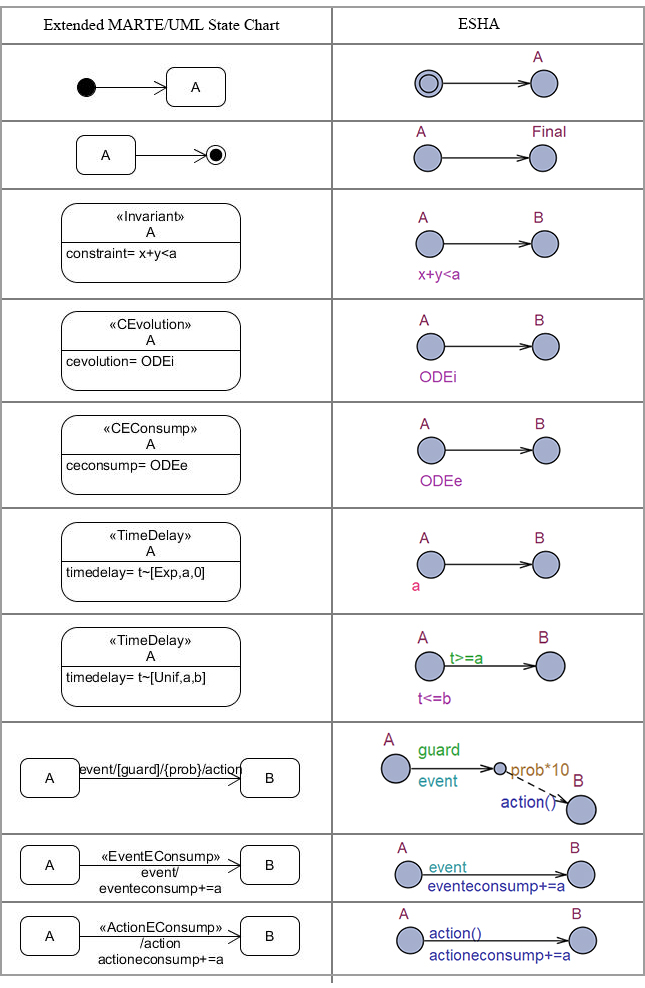
\includegraphics[width=3.7in]{mapping(new).jpg}
	\caption{扩展的MARTE/UML状态图-ESHA模型的映射规则}
	\label{SC2ESHA}
	\end{figure}
	
	由图中的映射关系可知,扩展的MARTE/UML状态图元素和ESHA模型元素在表达含义上具有一致性,为实现模型转换提供了依据。
	
	\textbf{示例}
	
	图\ref{example-trans}所示为一个简单的模型映射示例:一个加热器初始处于空闲状态,当接收到$on?$信号后,有$50\%$的概率进入$heat1$状态,$50\%$的概率进入$heat2$状态,且接收信号这一事件会产生2个单位的能耗;当加热器处在$heat1$状态时,每单位时间的能耗值为5,提供的加热功率为2,且加热4至5个单位时间后会再次返回空闲状态;当加热器处在$heat2$状态时,每单位时间的能耗值为10,提供的加热功率为5,同样地,在加热4至5个单位时间后会再次返回空闲状态。图\ref{trans-sc}为该示例对应的扩展MARTE/UML状态图,图\ref{trans-esha}为按照元素映射规则转换后的ESHA模型。
	
	\begin{figure}
	\centering
	\subfigure[扩展的MARTE/UML状态图]{
	\begin{minipage}[b]{0.4\textwidth}
	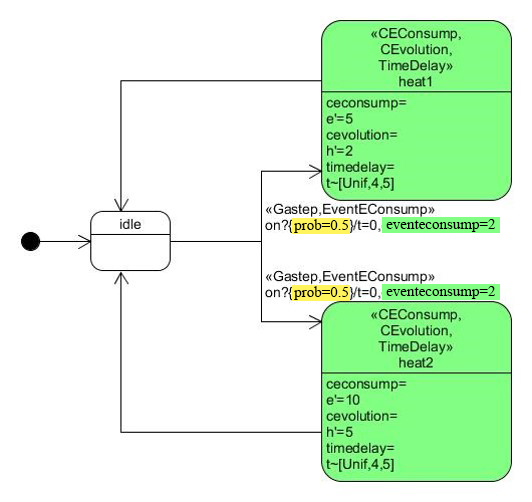
\includegraphics[width=1\textwidth]{example-trans.jpg} 
	\end{minipage}
	\label{trans-sc}
	}
	\subfigure[对应的UPPAAL-SMC ESHA模型]{
	\begin{minipage}[b]{0.4\textwidth}
	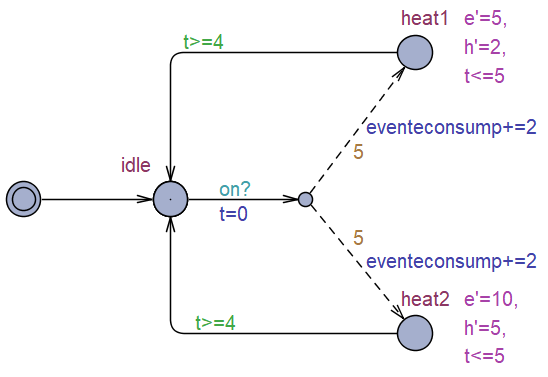
\includegraphics[width=0.8\textwidth]{example-trans.png} 
	\end{minipage}
	\label{trans-esha}
	}
	\caption{扩展的MARTE/UML状态图-ESHA模型的映射示例}
	\label{example-trans}
	\end{figure}

\subsection{模型转换伪代码}
	下面我们给出从扩展的MARTE/UML状态图到UPPAAL-SMC的ESHA模型转换的伪代码。转换的输入为扩展的MARTE/UML状态图,通过前述的元素映射规则,将状态图中的元素一一映射为ESHA模型的元素:对于一个迁移$\tau_{i}$,首先,对其源状态和目标状态进行类型判断,映射为对应的位置(若该状态已经转换为位置,则无需重复操作,从位置数组L中找到对应位置即可);接着,对迁移的$prob$进行判断,若$prob$值不等于1,说明此迁移为离散概率迁移,为该迁移设置一个Branch节点(若已设置则无需重复操作,从分支节点数组B中找到对应节点即可),并从迁移的源位置态到分支节点设置边$Edge_{i1}$,将触发事件、监护条件和概率对应到$Edge_{i1}$上,$prob \times 10$对应于$Probability Weight$。从分支节点到目标位置设置边$Edge_{i2}$,将执行效应和能耗函数对应到$Edge_{i2}$上。若$prob$值等于1,说明此迁移不存在概率选择,无需设置分支节点,从源位置到目标位置设置边$Edge_{i}$,并将迁移上的元素一一映射;对于源状态,按照映射规则将状态上的元素一一映射为位置上的元素。以下为模型转换的伪代码:
		
%\begin{breakalgo}	
\renewcommand{\algorithmicrequire}{\textbf{输入:}}
\renewcommand{\algorithmicensure}{\textbf{输出:}}
%\begin{algorithm}
	
	%\caption{扩展的MARTE/UML状态图-UPPAAL ESHA模型的转换}
	\begin{algorithmic}[1]
	\label{trans}
	\algsetup{linenosize=\small} \small
		\REQUIRE 扩展的MARTE/UML状态图 SC
		\ENSURE UPPAAL-SMC ESHA模型
		\STATE 数组L:已添加的location集合;数组S:记录状态s是否已添加对应的location 
		\STATE 数组B:已添加的Branch节点结合;
		\STATE 数组REC:记录$prob\not=1$的(s,evn,grd)是否已添加对应的Branch节点
		\STATE 数组E:已添加的Edge集合
		
		\FOR {$\tau_{i}$ in SC}
		 
		\IF {$S[\tau_{i}.src]==1$}	
		\STATE FIND $l_{i}$ for $\tau_{i}.src$ in L ~~~~\COMMENT{若源location已添加,则找到对应location}
		\ELSIF {$typeof(\tau_{i}.src)==initial$} 
   		\STATE SET $\tau_{i}.src$ --> initial location $l_{i}$
		\ELSIF {$typeof(\tau_{i}.src)==final$}
   		\STATE SET $\tau_{i}.src$--> final location $l_{i}$
		\ELSE 
   		\STATE SET $\tau_{i}.src$--> location $l_{i}$
		\ENDIF

		\IF {$S[\tau_{i}.tgt]==1$}	
		\STATE FIND $l_{j}$ for $\tau_{i}.tgt$ in L  ~~~~\COMMENT{若目标location已添加,则找到对应location}
		\ELSIF {$typeof(\tau_{i}.tgt)==initial$} 
   		\STATE SET $\tau_{i}.tgt$--> initial location $l_{j}$
		\ELSIF {$typeof(\tau_{i}.tgt)==final$}
   		\STATE SET $\tau_{i}.tgt$--> final location $l_{j}$
		\ELSE 
   		\STATE SET $\tau_{i}.tgt$--> location $l_{j}$
		\ENDIF

		\IF {$\tau_{i}.prob \not=1$}
		\IF {$REC[\tau_{i}.src,\tau_{i}.evn,\tau_{i}.grd]==1$}	
			\STATE FIND Branch $b_{i}$ in B  ~~~~\COMMENT{若存在概率分支且Branch节点已添加,则找到对应Branch节点}
			\STATE FIND Edge $Edge_{i1}$ in E
		\ELSE
			\STATE SET Branch $b_{i}$ ~~~~\COMMENT{若存在概率分支且Branch节点未添加,则添加对应Branch节点}
			\STATE SET Edge $Edge_{i1}$ FROM $l_{i}$ TO $b_{i}$
		\ENDIF
		\STATE SET $Edge_{i2}$ FROM $b_{i}$ TO $l_{j}$ 
		\STATE SET $\tau_{i}.prob \times 10$-->$Edge_{i2}.Probability Weight$ ~~~~\COMMENT{状态图中的prob表示概率,UPPAAL-SMC中的Probability Weight表示比率}
		\STATE SET $\tau_{i}.evn$-->$Edge_{i1}.sync$ ~~~~\COMMENT{离散概率分支下,迁移元素的对应转换}
		\STATE SET $\tau_{i}.grd$-->$Edge_{i1}.guard$
		\STATE SET $\tau_{i}.act$-->$Edge_{i2}.update$
		\STATE SET $\tau_{i}.eng$-->$Edge_{i2}.update$
		
		\ELSE		
		\STATE SET $Edge_{i}$ FROM $l_{i}$ TO $l_{j}$
		\STATE SET $\tau_{i}.evn$-->$Edge_{i}.sync$ ~~~~\COMMENT{无离散概率分支下,迁移上元素的对应转换}
		\STATE SET $\tau_{i}.grd$-->$Edge_{i}.guard$
		\STATE SET $\tau_{i}.act$-->$Edge_{i}.update$
		\STATE SET $\tau_{i}.eng$-->$Edge_{i}.update$
		\ENDIF

		\STATE SET $\tau_{i}.src.sname$-->$l_{i}.name$ ~~~~\COMMENT{状态上元素转换为location上元素}
		\STATE SET $\tau_{i}.src.inv$-->$l_{i}.invariant$
		\STATE SET $\tau_{i}.src.diff$-->$l_{i}.invariant$
		\STATE SET $\tau_{i}.src.eng$-->$l_{i}.invariant$
		\IF {$typeof(\tau_{i}.src.distr)==Exp$}	
			\STATE SET $\tau_{i}.src.distr.a$-->$l_{i}.Rate of Exponential$ ~~~~\COMMENT{指数时延概率分布,在UPPAAL-SMC中直接设置比率}
		\ELSIF {$typeof(\tau_{i}.src.distr)==Unif$}	
			\STATE SET $\tau_{i}.src.distr.a$-->$Edge_{i(i1)}.guard$ ~~~~\COMMENT{均匀时延概率分布,在UPPAAL-SMC中通过location上的invariant和迁移上的guard表示}
			\STATE SET $\tau_{i}.src.distr.b$-->$l_{i}.invariant$
		\ENDIF

		\ENDFOR
	\end{algorithmic}
%\end{algorithm}
%\end{breakalgo}	

\section{建模与分析方法的实现框架}
	Modana\citep{DBLP:conf/compsac/ChengWLD15,杜德慧2017一种面向}是我们自己设计、开发的建模和分析平台,意为“modeling”和“analysis”的融合,旨在提供一套完整的CPS建模、分析方法。Modana的核心思想在于:通过集成的方式实现不同模型间的协作,其中既包含同层模型,也包含跨层模型。同层异构模型,如可执行的PRISM\citep{Kwiatkowska2002PRISM}与Modelica\citep{Elmqvist1997Modelica}模型,可以通过协同仿真技术\citep{Blochwitz2012Functional}实现异构模型间的仿真;跨层模型,如设计模型(UML/MARTE)与可执行模型(马尔科夫链(Markov Chain, MC)\citep{施仁杰1992马尔科夫链基础及其应用}、随机混成自动机等),可以通过模型自动转换实现设计模型的仿真、验证。
	
	图\ref{modana}所示为Modana平台的体系结构,左侧为概念框架,从软件工程的角度,将MDD的系统设计方法归纳为四个抽象模块:图形化建模模块、模型转换模块,协同仿真模块及分析与验证模块。右侧为对应的平台实现,图形化建模支持本文提出的扩展MARTE/UML状态图、SHA,MC及Modelica模型;设计模型需要经过Modana模型转换器转换,才能执行仿真,而可执行模型SHA、MC、Modelica则直接进入仿真器。Modana集成了3种仿真器:UPPAAL,PRISM和JModelica,并实现了部分模型的协同仿真。最终,由Modana调用外部仿真器生成模拟路径,进入Modana统计模型检测器,并利用我们之前的工作——自适应统计模型检测方法\citep{杜德慧2017一种面向}进行模型的属性验证和分析。
	\begin{figure}[!t]
	\centering
	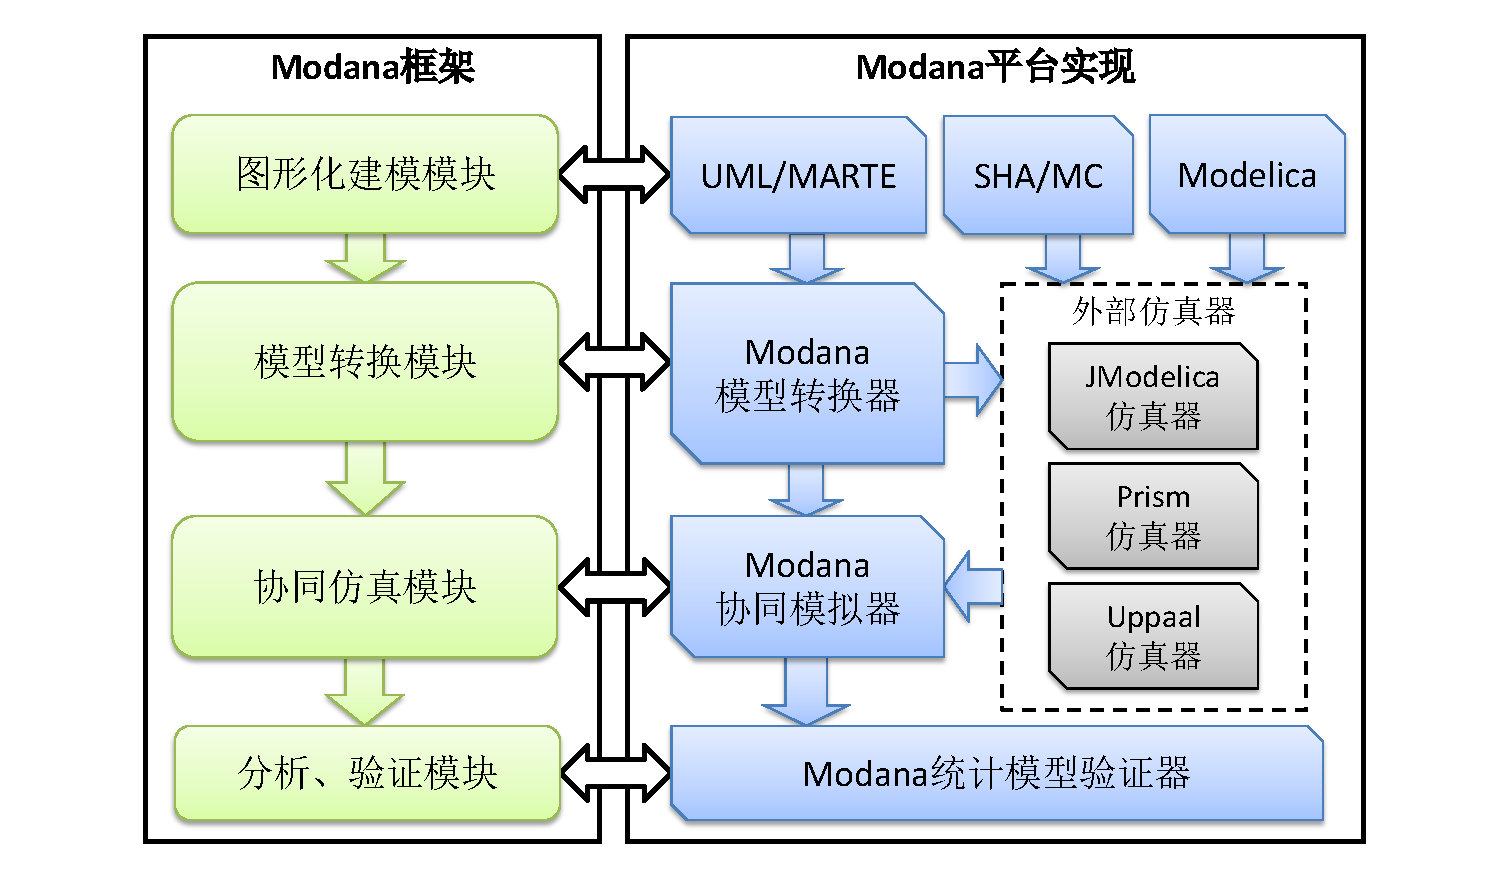
\includegraphics[width=4in]{modana.pdf}
	\caption{Modana体系结构}
	\label{modana}
	\end{figure}
	
	%基于Modana平台,可以实现本文提出的扩展的MARTE/UML状态图的建模以及模型转换为ESHA。
	%UPPAAL-SMC\citep{DBLP:journals/spe/BehrmannDLPY11,DBLP:journals/corr/abs-1207-1272}是时下最流行的模型检测工具之一,它提供了图形化建模SHA的功能,并利用统计模型检测方法(Stochastic Model Checking,SMC)实现对模型的定性、定量分析,且验证效率较高。

	基于3.3.3节中扩展的MARTE/UML状态图定义和4.1.1节中的ESHA定义,以及模型映射规则,在Modana平台的基础上,我们实现了扩展MARTE/UML状态图到ESHA的自动转换。利用Modana前端建模模块,可以实现扩展的MARTE/UML状态图的建模,并导出XML格式的模型文件。而UPPAAL-SMC的能耗随机混成自动机模型文件格式也为XML形式,模型转换实质上为两种XML文件对应节点的转换,这为实现扩展的MARTE/UML状态图到ESHA的转换提供了技术基础。
	
	\begin{figure}[!t]
	\centering
	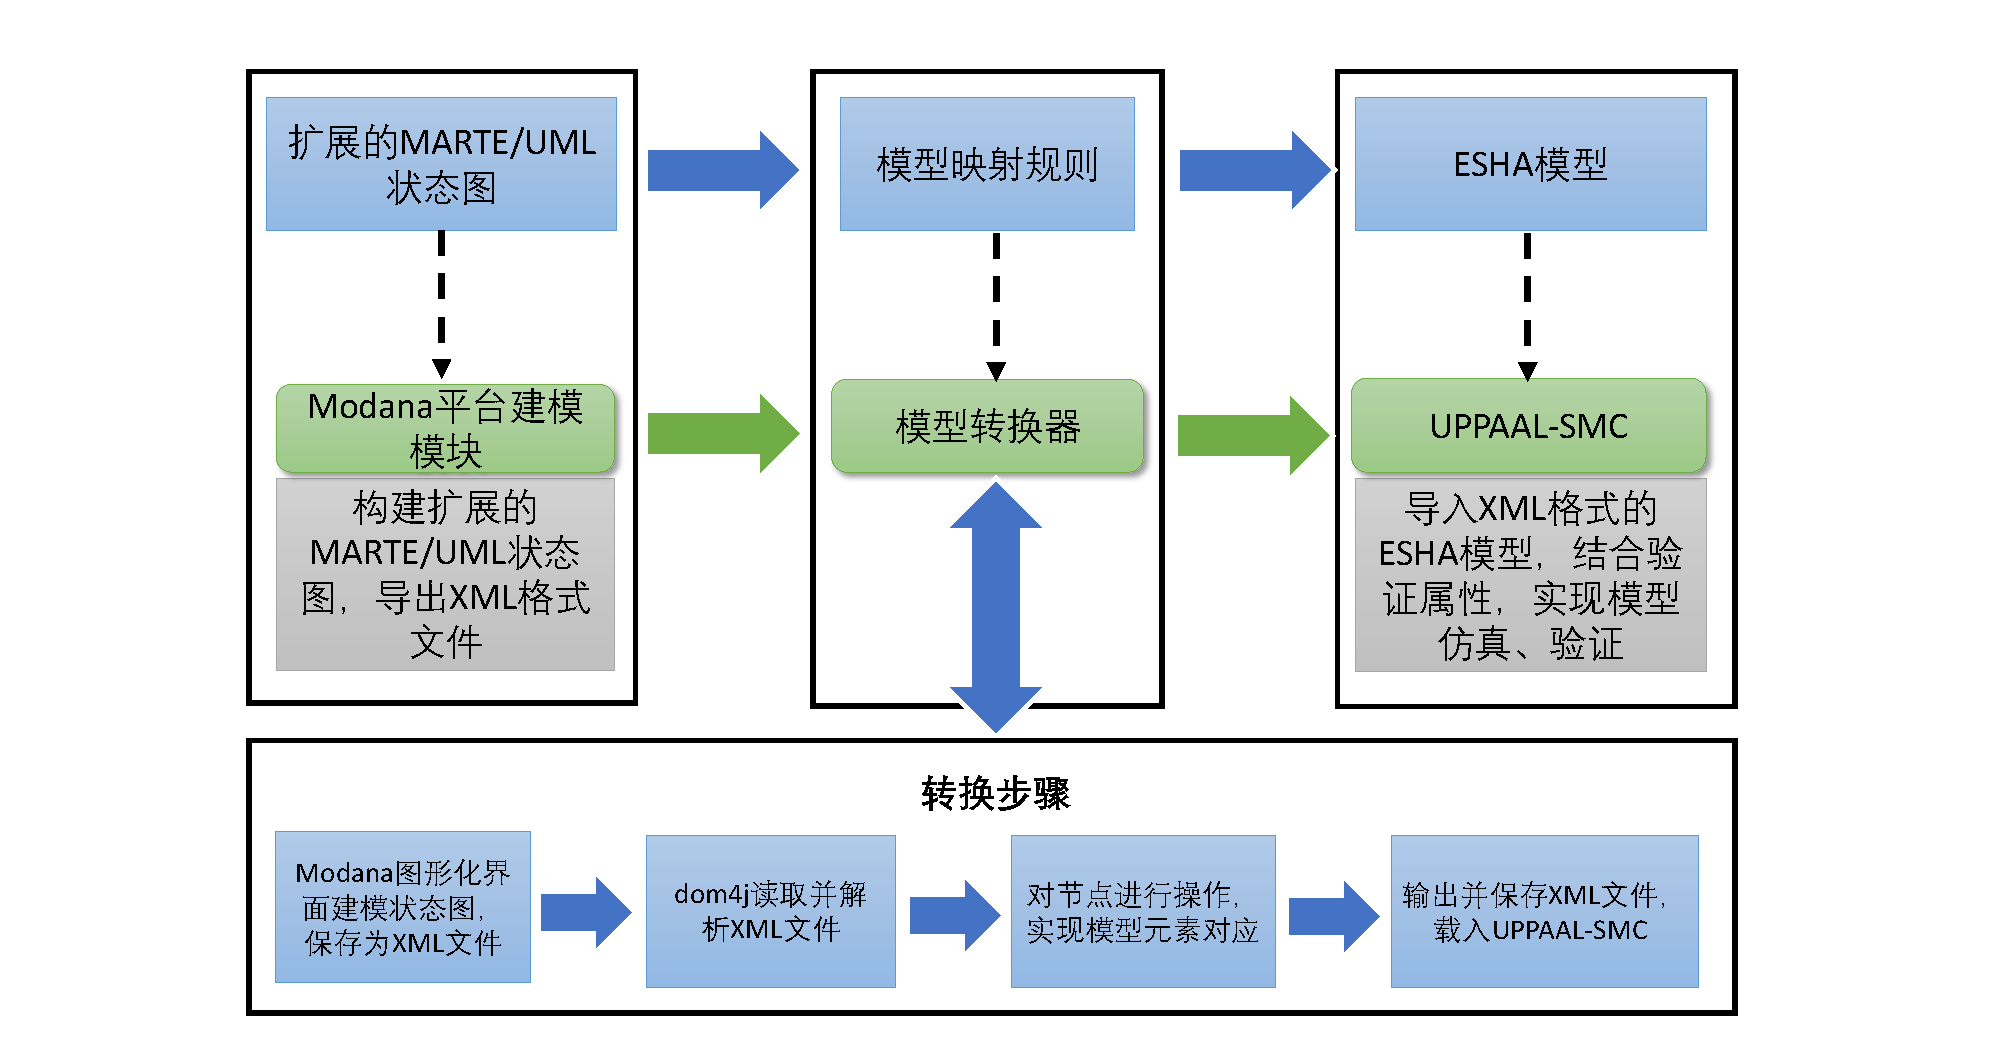
\includegraphics[width=4.6in]{tran.pdf}
	\caption{基于Modana和UPPAAL-SMC的实现框架}
	\label{tools}
	\end{figure}
	
	如图\ref{tools}所示,基于Modana和UPPAAL-SMC工具,可以实现本文提出的智能建筑能耗的建模与分析方法。
	
	在模型转换过程中,我们使用了dom4j来操作模型文件。dom4j是Java的一个XML API,可以用来读写XML文件。它可以实现建立XML文档,添加、修改、删除节点,以及格式化输出等功能。dom4j具有性能优异、功能强大且简单易用的优点,同时它也是一个开源库。本文基于Modana前端建模模块,使用dom4j读取扩展的MARTE/UML状态图XML文件,查询文件中的元素,通过序列化XML文档生成对应的ESHA模型文件,最后,载入UPPAAL-SMC中实现模型验证。具体步骤如下:
	\begin{itemize}
	\item 通过Modana前端建模模块绘制扩展的MARTE/UML状态图,并存储为XML文件;
	\item 使用dom4j读取扩展的MARTE/UML状态图的XML文件,查询XML节点,筛选出模型元素;
	\item 通过模型映射规则,修改XML节点,实现对应元素映射;
	\item 导出序列化XML文件,载入UPPAAL-SMC中,输入验证属性实现模型仿真、验证。
	\end{itemize}
	
	
	%\begin{itemize}
	%\item 状态映射:初始状态对应于初始位置;终止状态对应于终止位置;Invariant衍型的状态,其constraint的不变式表达式对应于ESHA位置上的不变式约束;CEvolution衍型的状态,其cevolution的微分表达式对应于ESHA位置上的微分等式;CEConsump衍型的状态,其ceconsump的能耗微分表达式对应于ESHA位置上的能耗微分等式;TimeDelay衍型的状态,其timedelay的时延概率分布对应于ESHA位置上的时钟迁移约束;
	%\item 迁移映射:状态图中迁移的源状态和目标状态分别对应于ESHA中的源位置和目标位置,警备条件、触发事件、执行效应以及迁移概率也都一一对应;在状态图中,一个EventEconsump衍型的迁移,其触发事件所消耗的能量在ESHA中被定义为执行效应中对eventeconsump变量的重新赋值;一个ActionEconsump衍型的迁移,其执行效应所消耗的能量在ESHA中被定义为执行效应中对actioneconsump变量的重新赋值。
	%\end{itemize}
	
\section{本章小结}
	尽管MARTE/UML模型可以实现系统的多视图建模,但由于其半形式化的特点,无法实现系统的仿真、验证。因此,为了对系统模型进行进一步分析,本章在随机混成自动机的基础上,提出了能耗随机混成自动机的概念,支持系统能耗的显式建模,且可以利用统计模型检测方法对其进行系统属性的高效验证。为了将MARTE/UML模型和ESHA联系起来,我们给出了扩展的状态图到ESHA的映射规则和算法,并基于我们的Modana工具和模型验证工具UPPAAL-SMC,给出了本文所提的智能建筑能耗建模与分析方法的实现框架。


